\documentclass{article}
\usepackage[top=2cm,bottom=2cm,left=2cm,right=2cm]{geometry}
\usepackage{amsmath, amsthm}
\usepackage{tikz}
\usepackage{hyperref}

\usepackage{datetime}
\newdateformat{petsa}{\the\day\ \shortmonthname[\the\month] \the\year}

\theoremstyle{plain}
\newtheorem{definition}{Definition}[section]
\newtheorem{theorem}{Theorem}[section]
\newtheorem{lemma}[theorem]{Lemma}
\newtheorem{conjecture}[theorem]{Conjecture}

\theoremstyle{remark}
\newtheorem*{remark}{Remark}

\title{Description of \texttt{treedrawing}}
\author{poypoyan}
\date{\petsa\today}

\begin{document}

\maketitle

\begin{abstract}
This note contains an overview of my Github repo \texttt{treedrawing} \cite{treedrawing}, which is a naive algorithm that neatly draws rooted trees.
\end{abstract}

\section{Definitions}
We start by introducing some standard and non-standard terminologies:
\begin{definition}
A \textbf{rooted tree} is a triple $T=(V, E, r)$ where $(V, E)$ is a tree (a graph without cycles), and $r \in V$ is called the \textbf{root}.
\end{definition}
\begin{remark}
We adopt terminologies from computer science: we call $V$ the set of \textbf{nodes} (instead of vertices), and $E$ the set of \textbf{branches} (instead of edges).
\end{remark}
\begin{definition}
For nodes $x, y \in V$ connected by a branch, $x$ is the \textbf{parent} of $y$ and $y$ is a \textbf{child} of $x$ if $x$ has closer path to the root than $y$. 
\end{definition}
\begin{definition}
A \textbf{leaf} is a node that does not have a child.
\end{definition}
\begin{definition}
A non-root node is \textbf{minor} iff it is the only child of its parent and it has exactly one child node. A node is \textbf{major} iff it is the root or it is not minor. 
\end{definition}
\begin{definition}
The \textbf{sub-rooted tree} by a major node $x \in V$ is a rooted tree $T'=(V', E', x)$ consisting of $x$ itself (as root) and all of its the `descendant' nodes.
\end{definition}
\begin{remark}
(1) The sub-rooted tree by the root node is the whole rooted tree. (2) The sub-rooted tree by the leaf node is the trivial branch-less tree with itself as the only node.
\end{remark}
\begin{definition}\label{weight}
The \textbf{weight} of a major node is the number of major nodes of the sub-rooted tree by that node. The weight of a minor node is 0.
\end{definition}
\begin{remark}
The weight of every leaf node is 1.
\end{remark}

We show the converse of the last sentence in Definition \ref{weight}: all nodes of weight 0 are minor. This is equivalent to the statement that all major nodes have weights of at least 1. This is indeed the case because the major node itself is contained in the sub-rooted tree by itself. In conclusion, a node is minor iff its weight is 0.

To aid in understanding the concepts, an example rooted tree is provided in Figure \ref{rooted-tree}.

\begin{figure}[htbp]
	\centering
	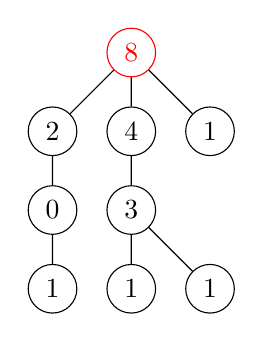
\begin{tikzpicture}[nodes = {draw, circle}]
		\node [red] {8} [sibling distance = 1cm, level distance = 1cm]
		child {node {2}
			child {node {0}
				child {node {1}}
			}
		}
		child {node {4}
			child {node {3} [sibling distance = 2cm]
				child {node [xshift = 1cm] {1}}
				child {node {1}}
			}
		}
		child {node {1}};
	\end{tikzpicture}
	\caption{Example rooted tree with red-colored node as the root. The number in node indicates its weight.}
	\label{rooted-tree}
\end{figure}

\section{Algorithm Description}
The algorithm consists of three main functions that are executed in order: (1) \texttt{analyzeNode}, which records relevant information for each node recursively, (2) \texttt{setInitCoord}, which sets initial coordinates to each node recursively, and (3) \texttt{fixCoord}, which fixes coordinates of nodes so that there are no nodes with same location.

\subsection{Function \texttt{analyzeNode}}
The main input \footnote{Throughout this paper, we only mention the `important' inputs. Other inputs are instead mentioned in \texttt{example.py} comments.} of the algorithm is any data with a structure of rooted tree. Note that nodes in the input data must be \textit{labelled}. What the \texttt{analyzeNode} function mainly does is to perform tree traversal on the data and record the following information:

\begin{itemize}
	\item \texttt{connecNodes} is an array of arrays of natural numbers. An index \texttt{idx} in \texttt{connecNodes[idx]} corresponds to a node (with \texttt{idx = 0} being the root). Now \texttt{connecNodes[idx]} itself is the array of indices that correspond to the \textit{children} of the \texttt{idx} node. If the \texttt{idx} node is a leaf, then \texttt{connecNodes[idx]} is the empty array.
	\item \texttt{labelDict} is a function that aligns node \textit{labels} (strings) to indices for \texttt{connecNodes}, \texttt{weightNodes}, and \texttt{majorNodes}.
	\item \texttt{weightNodes} is an array of natural numbers. Like in \texttt{connecNodes}, an index \texttt{idx} in \texttt{weightNodes[idx]} corresponds to a node (with \texttt{idx = 0} being the root). Now \texttt{weightNodes[idx]} itself is the weight of the \texttt{idx} node.
	\item \texttt{majorNodes} is an array of objects. Like in \texttt{connecNodes}, an index \texttt{idx} in \texttt{majorNodes[idx]} corresponds to a node (with \texttt{idx = 0} being the root). Now for major nodes, \texttt{majorNodes[idx]} itself is the array of major nodes along the (unique) path from the root to the \texttt{idx} node (\texttt{idx} itself excluded). Since the root has no parent, \texttt{majorNodes[0]} is always the empty array. For minor nodes, \texttt{majorNodes[idx]} is the \textit{null} object.
\end{itemize}

\subsection{Function \texttt{setInitCoord}}
As the name says, this function sets initial coordinates for each node. These coordinates are stored in \texttt{coordNodes}. The root's coordinate is always set to $(0,0)$. The major nodes are always set to coordinates of upright square lattice (see Figures \ref{lattice} and \ref{setinitcoord}). We let \texttt{dist} the distance between consecutive horizontal/vertical points in the upright square lattice; it is hard-coded to $1.0$. Aside from the above outputs of \texttt{analyzeNode} except \texttt{labelDict}, the other relevant input is \texttt{outDir}, the direction of `growth' of rooted tree. For the following discussion, we set \texttt{outDir = `D'} (downward direction).

\begin{figure}[htbp]
	\centering
	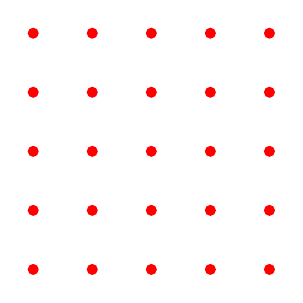
\begin{tikzpicture}
		\foreach \i in {0,...,4}
		\foreach \j in {0,...,4}
		\node[circle, minimum width = 4pt, inner sep = 0pt, fill = red] at (\i * 0.75 cm, \j * 0.75 cm) {};
	\end{tikzpicture}
	\caption{Upright square lattice. The middlemost point would be the origin.}
	\label{lattice}
\end{figure}

For each major node $x$ with one child node, minor nodes are traversed until encountering another major node $y$. The coordinate for $y$ is set to one \texttt{dist} directly \textit{below} (since \texttt{outDir = `D'}) the coordinate of $x$. On the other hand, the coordinates of minor nodes between $x$ and $y$ are `squeezed' between the coordinates of $x$ and $y$ at equal distance to each other. Now $y$ either has no child or has multiple children. The former means unwinding the recursion. For the latter, $y$'s children are all one \texttt{dist} below $y$. Now the x-coordinate of the children depends on their weights: the child with highest weight is placed directly below $y$, then the child with next highest weight is placed one \texttt{dist} away from the closest child. The placement of children swings (e.g. center, left, right, left, $\ldots$) and goes \textit{away} from the child with highest weight. All of this is visualized in Figure \ref{setinitcoord}.

\begin{figure}[htbp]
	\centering
	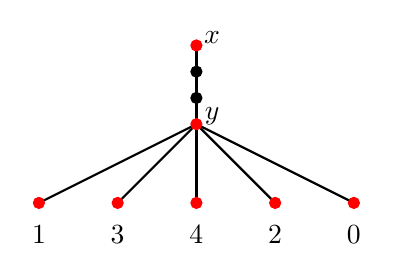
\begin{tikzpicture}[nodes = {draw, circle, minimum width = 4pt, inner sep = 0pt}]
		\draw[-, thick = 2pt] (0 cm, 0 cm) -- (0 cm, -2 cm);
		\draw[-, thick = 2pt] (0 cm, -1 cm) -- (-1 cm, -2 cm);
		\draw[-, thick = 2pt] (0 cm, -1 cm) -- (1 cm, -2 cm);
		\draw[-, thick = 2pt] (0 cm, -1 cm) -- (-2 cm, -2 cm);
		\draw[-, thick = 2pt] (0 cm, -1 cm) -- (2 cm, -2 cm);
		\node[color = red, fill = red] at (0 cm, 0 cm) {};
		\node[fill = black] at (0 cm, -0.333 cm) {};
		\node[fill = black] at (0 cm, -0.667 cm) {};
		\node[color = red, fill = red] at (0 cm, -1 cm) {};
		\node[color = red, fill = red] at (0 cm, -2 cm) {};
		\node[color = red, fill = red] at (-1 cm, -2 cm) {};
		\node[color = red, fill = red] at (1 cm, -2 cm) {};
		\node[color = red, fill = red] at (-2 cm, -2 cm) {};
		\node[color = red, fill = red] at (2 cm, -2 cm) {};
		\node[draw = none] at (0.2 cm, 0.1 cm) {$x$};
		\node[draw = none] at (0.2 cm, -0.9 cm) {$y$};
		\node[draw = none] at (0 cm, -2.4 cm) {4};
		\node[draw = none] at (-1 cm, -2.4 cm) {3};
		\node[draw = none] at (1 cm, -2.4 cm) {2};
		\node[draw = none] at (-2 cm, -2.4 cm) {1};
		\node[draw = none] at (2 cm, -2.4 cm) {0};
	\end{tikzpicture}
	\caption{Initial coordinates; branches are drawn for clarity. Major nodes are red and minor nodes are black. Example weights of bottom nodes are also indicated.}
	\label{setinitcoord}
\end{figure}

The reasoning behind placement of children is aesthetics: the central path from root should have the most major nodes, and the sub-rooted trees that branch away from the central path should be minimal.

\subsection{Function \texttt{fixCoord}}
The problem with the previous function is that several major nodes will have the same coordinates. This is what \texttt{fixCoord} fixes. For each major node $x$, let $y$ be first index in \texttt{coordNodes} such that \texttt{coordNodes[x] = coordNodes[y]}. If $x \ne y$, then a duplicate coordinate is found.

Using \texttt{majorNodes}, the two major nodes that have the same parent and splits the path from root to $x$ and the path from root to $y$ are determined. The indices of that major node for $x$ and for $y$ are stored at \texttt{splitNodeA} and \texttt{splitNodeB} (let's say respectively). If for example \texttt{weight[splitNodeA] > weight[splitNodeB]}, then the whole sub-rooted tree by \texttt{splitNodeB} must move \textit{away} from the central path from root (and vice versa). This also means that the coordinate of $y$ must move. How many \texttt{dist} to move? The whole sub-rooted tree by \texttt{splitNodeB} must move away until the coordinate of $y$ is not equal to the coordinates of $x$ and all siblings of $x$.

After the movement, the next $x$ is checked. Looping through major nodes is continued until no duplicate coordinate is found, which means the function is done.

\section{Notes for Programmer}
The main output of the algorithm is the final coordinates of each node, \texttt{coordNodes}. On the other hand, the drawing of branches is actually not an output! This means that the drawing of branches must be done in a separate code/program, although I have the simple `straight line' branches (as seen in Figures \ref{setinitcoord} and \ref{interbranch}) in mind.

Since the coordinate of root node and \texttt{dist} are hard-coded to $(0,0)$ and $1.0$, respectively, one can `customize' the coordinates in the following manner: $$\mathbf{r} + s * \texttt{coordNodes[i]}$$
for all nodes $i$, where $\mathbf{r}$ is the actual root node coordinate and $s$ is the scalar.

Lastly, intersecting branches in a manner like in Figure \ref{interbranch} may occur.

\begin{figure}[htbp]
	\centering
	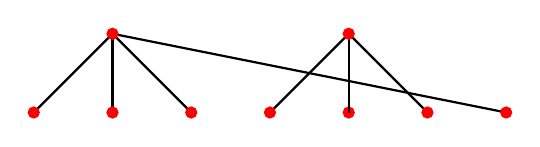
\begin{tikzpicture}[nodes = {draw, circle, minimum width = 4pt, inner sep = 0pt}]
		% sub-rooted tree 1
		\draw[-, thick = 2pt] (-2 cm, 0 cm) -- (-2 cm, -1 cm);
		\draw[-, thick = 2pt] (-2 cm, 0 cm) -- (-3 cm, -1 cm);
		\draw[-, thick = 2pt] (-2 cm, 0 cm) -- (-1 cm, -1 cm);
		\draw[-, thick = 2pt] (-2 cm, 0 cm) -- (3 cm, -1 cm);
		\node[color = red, fill = red] at (-2 cm, 0 cm) {};
		\node[color = red, fill = red] at (-2 cm, -1 cm) {};
		\node[color = red, fill = red] at (-3 cm, -1 cm) {};
		\node[color = red, fill = red] at (-1 cm, -1 cm) {};
		\node[color = red, fill = red] at (1 cm, -1 cm) {};
		% sub-rooted tree 2
		\draw[-, thick = 2pt] (1 cm, 0 cm) -- (0 cm, -1 cm);
		\draw[-, thick = 2pt] (1 cm, 0 cm) -- (1 cm, -1 cm);
		\draw[-, thick = 2pt] (1 cm, 0 cm) -- (2 cm, -1 cm);
		\node[color = red, fill = red] at (1 cm, 0 cm) {};
		\node[color = red, fill = red] at (0 cm, -1 cm) {};
		\node[color = red, fill = red] at (2 cm, -1 cm) {};
		\node[color = red, fill = red] at (3 cm, -1 cm) {};
	\end{tikzpicture}
	\caption{The right sub-rooted tree is sandwiched between two children of the left sub-rooted tree.}
	\label{interbranch}
\end{figure}

\bibliographystyle{plain}
\bibliography{treedrawing}
\end{document}